\documentclass[12pt,a4paper]{article}
\usepackage[english]{babel}
\usepackage[utf8]{inputenc}
\usepackage{amssymb,amsmath}
\usepackage[all]{xy}
\usepackage{url}
\usepackage{graphicx}
\usepackage{color}
\newcommand{\angstrom}{\textup{\AA}}
\color{black}
\usepackage{geometry}
\usepackage[autostyle]{csquotes}
\usepackage{tikz}
\usetikzlibrary{bayesnet}
\def\UrlBreaks{\do\/\do-}
\usepackage{dcolumn}
\usepackage{booktabs}
\usepackage{tikz}
\usetikzlibrary{positioning,shapes,arrows}
\newcolumntype{M}[1]{D{.}{.}{1.#1}}
\usepackage{upquote} % Upright quotes for verbatim code
\usepackage{fancyvrb} % verbatim replacement that allows latex
\usepackage{float}

\usepackage{amsmath}
\usepackage{algorithm}
\usepackage[noend]{algpseudocode}
\usepackage{listings}
\makeatletter
\def\BState{\State\hskip-\ALG@thistlm}
\makeatother

\geometry{
	a4paper,
 	left=15mm,
 	right=15mm,
 	top=10mm,
 	bottom=15mm
}

\DefineVerbatimEnvironment{Highlighting}{Verbatim}{commandchars=\\\{\}}

\newcommand{\VerbatimStringTok}[1]{\textcolor[rgb]{0.25,0.44,0.63}{{#1}}}



\begin{document}
\title{State-of-the-art Chinese Word Segmentation with Bi-LSTMs}
\author{Michał Ostyk-Narbutt (1854051)\\Prof. Roberto Navigli \\ Natural Language Processing Homework 1}

\maketitle


\begin{center}

\includegraphics[width=0.5\textwidth]{img/sapienza_logo.jpg}
\end{center}
\maketitle
\tableofcontents
\clearpage
\section{Introduction}
\section{Model}
\section{Results}
\section{Conclusion}

%
%
%\begin{figure}[H]
%\begin{center}
%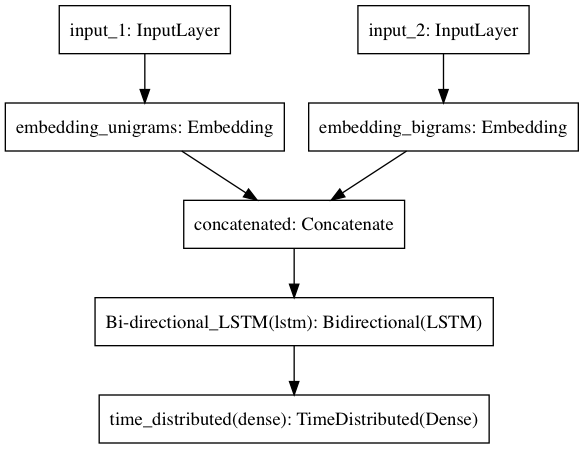
\includegraphics[width=0.7\columnwidth, angle = 0]{../report_images/model.png}
%\end{center}
%\caption{Keras model.}
%\label{img:clip}
%\end{figure}
The student has to deliver via the Google form:
a link to the Gitlab shared project with the source code and any additional data needed to run the software
a paper of up to 4 pages (+infinite pages for references, images, tables, graphs, etc.) including: a brief introduction to the project problem, a brief state of the art, an illustration of the methods/approach/techniques (min. 1 page), a quantitative (and ideally a small qualitative) evaluation of the system, some analysis of the results.
\\\\\




Algorithm \ref{euclid} depicts the overall procedure of training.
\begin{algorithm}
\caption{PPO with Clipped Objective }\label{euclid}
\begin{algorithmic}[1]
\item Collect a batch of $N$ (multiple of the mini-batch size) transitions from parallel environments \newline (state, action, log-probabilities,a reward, done-mask (0 if terminal), V(s) (value of the state for each state).
\item Calculate the returns for the batch using GAE
\item Calculate: advantage = returns - values
\item For $e$ epochs: \emph{loop}:
\begin{algorithmic}[1]
\item Sample through enough random mini-batches to cover all data.
\item Pass state into network, obtain action, value of state', entropy and new-log-probabilities.
\item Calculate the surrogate policy loss and MSE value loss.
\item Backpropagate the loss through the network using SGD.
\end{algorithmic}
\item 5. Repeat above until converged.
\end{algorithmic}
\end{algorithm}





\begin{thebibliography}{1}

\bibitem{code} \url{https://github.com/Ostyk/Chinese-LSTM}




\end{thebibliography}

\end{document}
